\section{Reasoning Techniques in LLMs}
\begin{frame}[allowframebreaks]{}
    \LARGE Reasoning Techniques in LLMs
\framebreak
    \begin{figure}[h]
        \centering
        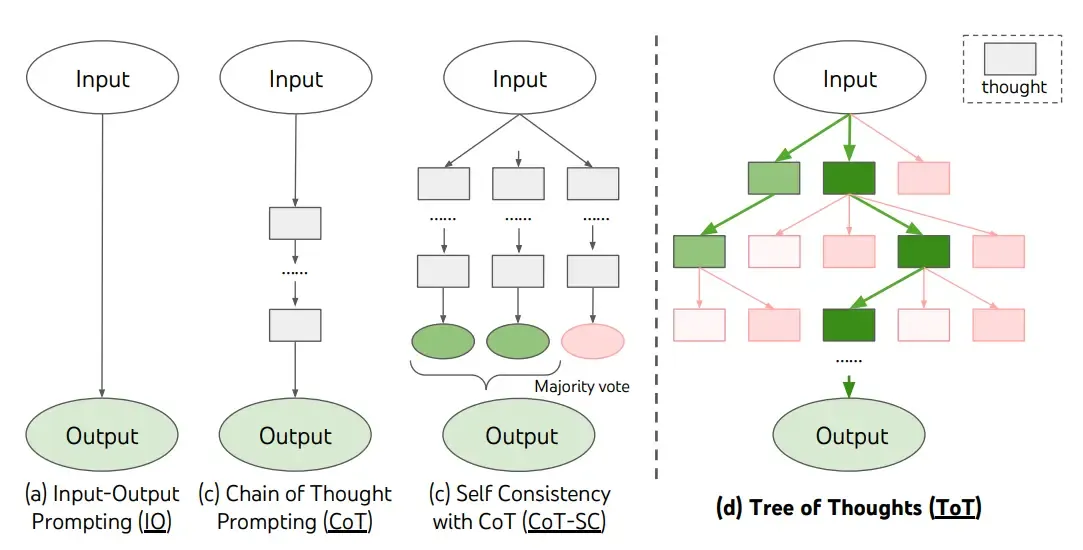
\includegraphics[width=\textwidth,height=0.9\textheight,keepaspectratio]{images/lrm+moe/reasoning-techniques.png}
    \end{figure}
\end{frame}

\subsection{Chain-of-Thought (CoT) Prompting}
\begin{frame}[allowframebreaks]{Chain-of-Thought (CoT) Prompting}
    \begin{itemize}
        \item \textbf{What is CoT?}
        \begin{itemize}
            \item A prompting technique that encourages LLMs to generate intermediate reasoning steps before arriving at a final answer.
            \item Helps models to break down complex problems into manageable parts.
        \end{itemize}
        \item \textbf{How it works:}
        \begin{itemize}
            \item Instead of asking for a direct answer, the prompt includes examples that show the reasoning process.
            \item The model is guided to think step-by-step, mimicking human-like reasoning.
        \end{itemize}
    \framebreak
        \item \textbf{Benefits:}
        \begin{itemize}
            \item Improves accuracy on tasks requiring multi-step reasoning, such as math problems or logical puzzles.
            \item Makes the model's reasoning process more transparent, allowing users to follow its logic.
        \end{itemize}
        \item \textbf{Example:}
        \begin{itemize}
            \item Instead of asking "What is 24 divided by 6?", the prompt might be "To find 24 divided by 6, we can think: 6 goes into 24 how many times? Let's break it down step by step."
        \end{itemize}
    \end{itemize}
    % \framebreak
    % \begin{figure}[h]
    %     \centering
    %     \includegraphics[height=0.8\textheight,width=\textwidth,keepaspectratio]{images/lrm+moe/cot-prompting.png}
    % \end{figure}
\end{frame}

\begin{frame}[allowframebreaks]{Few-shot CoT Prompting}
    \begin{itemize}
        \item \textbf{What is Few-shot CoT?}
        \begin{itemize}
            \item A variant of CoT prompting that provides a few examples of reasoning steps before the actual question.
            \item Helps the model learn the reasoning pattern from the examples.
        \end{itemize}
        \item \textbf{How it works:}
        \begin{itemize}
            \item The prompt includes several examples of problems and their step-by-step solutions.
            \item The model uses these examples to understand how to approach the new problem.
        \end{itemize}
    \framebreak
        \item \textbf{Benefits:}
        \begin{itemize}
            \item Enhances the model's ability to generalize from examples, improving performance on similar tasks.
            \item Reduces the need for extensive training on specific reasoning tasks.
        \end{itemize}
        \item \textbf{Example:}
        \begin{itemize}
            \item The prompt might include examples like "If 6 times 4 equals 24, then what is 6 times 5?" followed by the reasoning steps leading to the answer.
            \item The model learns to apply similar reasoning to new problems presented in the same format.
        \end{itemize}
    \end{itemize}
\end{frame}


\begin{frame}[allowframebreaks]{Zero-shot CoT Prompting}
    \begin{itemize}
        \item \textbf{What is Zero-shot CoT?}
        \begin{itemize}
            \item A variant of CoT prompting where the model is prompted to reason through a problem without any prior examples.
            \item The model generates its own reasoning steps based on the problem statement.
        \end{itemize}
        \item \textbf{How it works:}
        \begin{itemize}
            \item The prompt directly asks the model to think through the problem step-by-step, without providing specific examples.
            \item The model relies on its training to generate a logical sequence of reasoning.
        \end{itemize}
    \framebreak
        \item \textbf{Benefits:}
        \begin{itemize}
            \item Useful for novel problems where no examples are available.
            \item Encourages the model to apply its learned reasoning skills flexibly.
        \end{itemize}
        \item \textbf{Example:}
        \begin{itemize}
            \item The prompt might be "To solve the problem of how many apples Alice has after giving some to Bob, think step-by-step about what happens when she gives away apples."
            \item The model generates its own reasoning steps based on the prompt.
        \end{itemize}
    \end{itemize}
    \framebreak
    \begin{figure}[h]
        \centering
        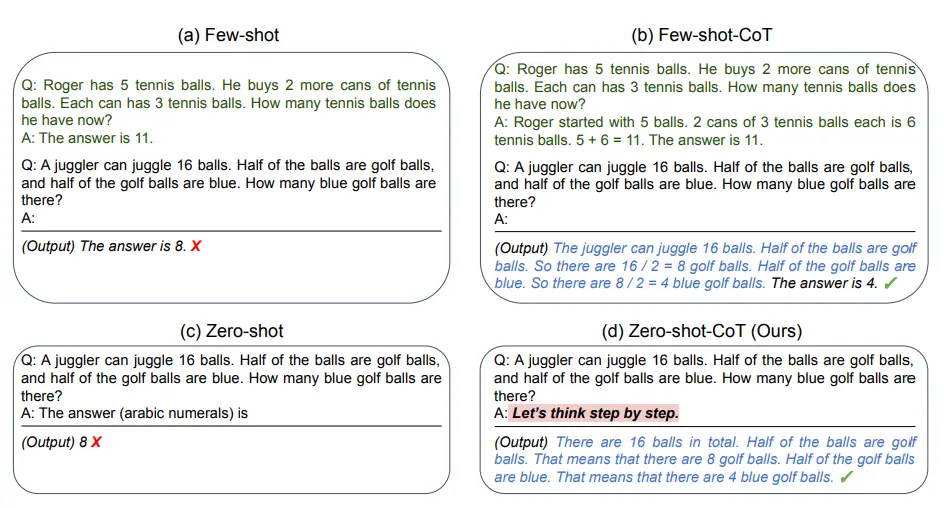
\includegraphics[height=0.8\textheight,width=\textwidth,keepaspectratio]{images/lrm+moe/few-shot_zero-shot.png}
        \caption*{Comparison of Few-shot and Zero-shot CoT Prompting. Source: \href{https://arxiv.org/abs/2210.03493}{Zhang et al. (2022)}}
    \end{figure}
\end{frame}


\begin{frame}[allowframebreaks]{Auto-CoT Prompting}
    \begin{figure}[h]
        \centering
        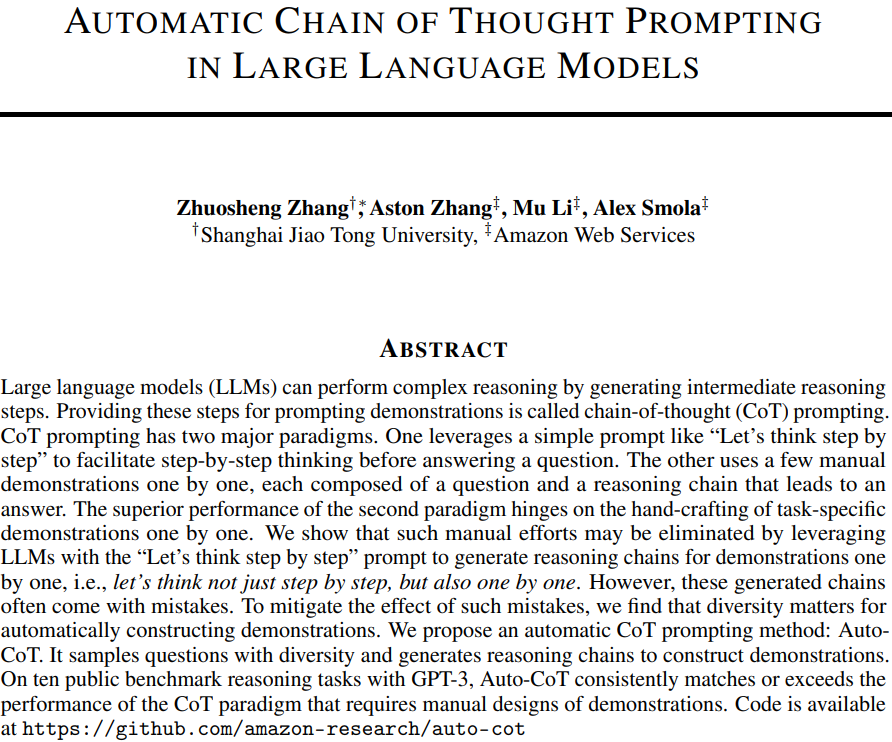
\includegraphics[height=0.9\textheight,width=\textwidth,keepaspectratio]{images/lrm+moe/paper-auto-cot.png}
    \end{figure}
    \begin{itemize}
        \item \textbf{What is Auto-CoT?}
        \begin{itemize}
            \item An automated approach to generating Chain-of-Thought prompts.
            \item Uses algorithms to create reasoning steps based on the problem context.
        \end{itemize}
        \item \textbf{How it works:}
        \begin{itemize}
            \item The system analyzes the problem and automatically generates a sequence of reasoning steps.
            \item This can be done using techniques like reinforcement learning or heuristic methods.
        \end{itemize}
    \framebreak
        \item \textbf{Benefits:}
        \begin{itemize}
            \item Reduces the manual effort required to create effective CoT prompts.
            \item Can adapt to a wide range of problems without needing specific examples.
        \end{itemize}
        \item \textbf{Example:}
        \begin{itemize}
            \item The system might take a problem like "If Alice has 3 apples and gives 2 to Bob, how many does she have left?" and automatically generate reasoning steps like "Start with 3 apples, subtract 2 apples given to Bob, and conclude with the remaining number of apples."
        \end{itemize}
    \end{itemize}
    \framebreak
    \begin{figure}[h]
        \centering
        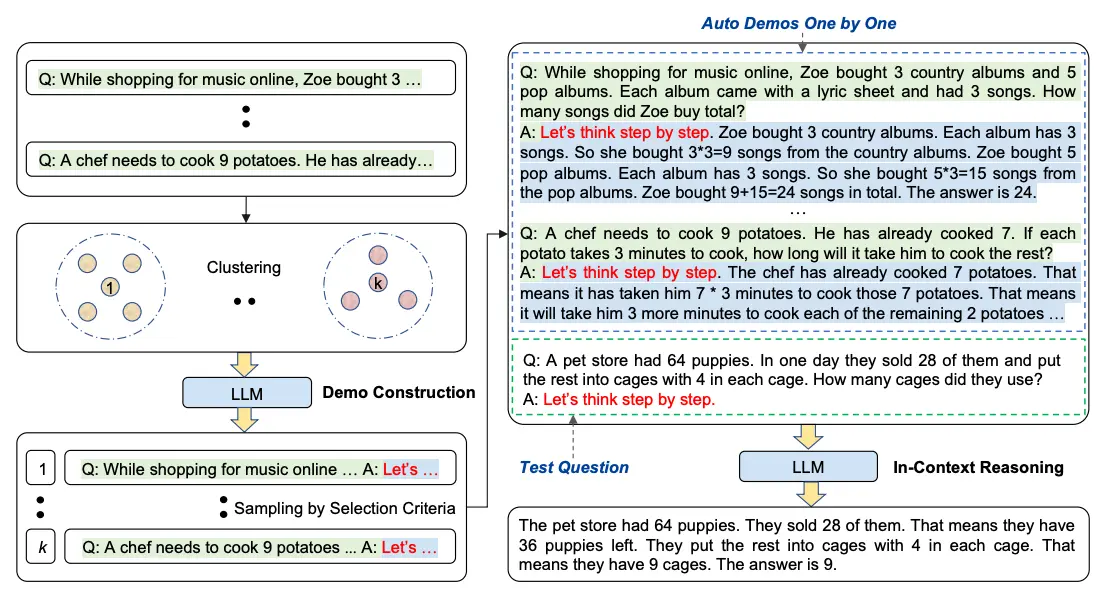
\includegraphics[height=0.8\textheight,width=\textwidth,keepaspectratio]{images/lrm+moe/auto-cot.png}
        \caption*{Auto-CoT Prompting. Source: \href{https://arxiv.org/abs/2210.03493}{Zhang et al. (2022)}}
    \end{figure}
    \framebreak
    \begin{figure}[h]
        \centering
        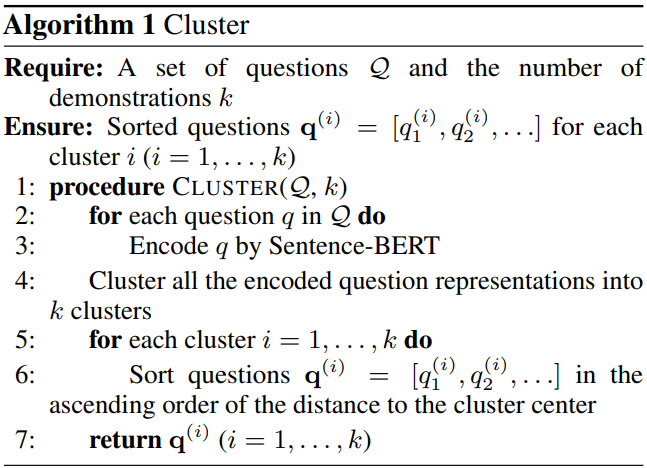
\includegraphics[height=0.9\textheight,width=\textwidth,keepaspectratio]{images/lrm+moe/algo-auto-cot-cluster.png}
    \end{figure}
    \framebreak
    \begin{figure}[h]
        \centering
        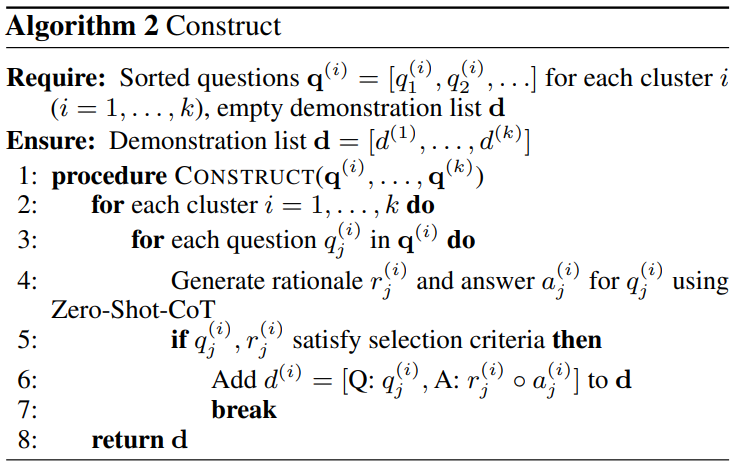
\includegraphics[height=0.9\textheight,width=\textwidth,keepaspectratio]{images/lrm+moe/algo-auto-cot-construct.png}
    \end{figure}
\end{frame}


\subsection{Tree-of-Thought (ToT) Reasoning}
\begin{frame}[allowframebreaks]{Tree-of-Thought (ToT) Reasoning}
    \begin{figure}[h]
        \centering
        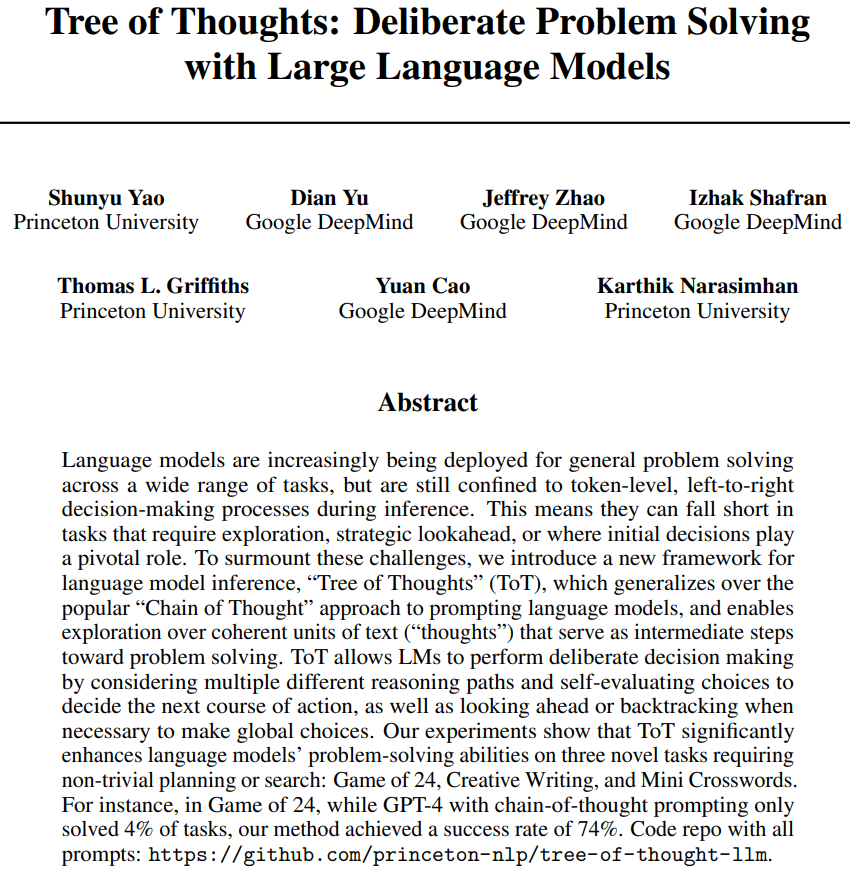
\includegraphics[height=0.9\textheight,width=\textwidth,keepaspectratio]{images/lrm+moe/paper-tot.png}
    \end{figure}
    \begin{itemize}
        \item \textbf{What is ToT?}
        \begin{itemize}
            \item A reasoning technique that structures the thought process as a tree, allowing for exploration of multiple reasoning paths.
            \item Each node in the tree represents a step in the reasoning process, and branches represent different possible paths or decisions.
        \end{itemize}
        \item \textbf{How it works:}
        \begin{itemize}
            \item The model generates a tree structure where each branch represents a different reasoning path.
            \item The model can explore multiple paths simultaneously, evaluating the outcomes of each.
        \end{itemize}
    \framebreak
        \item \textbf{Benefits:}
        \begin{itemize}
            \item Allows for more complex reasoning by considering multiple possibilities at once.
            \item Helps the model avoid getting stuck in a single line of reasoning, improving problem-solving capabilities.
        \end{itemize}
        \item \textbf{Example:}
        \begin{itemize}
            \item For a problem like "If Alice has 3 apples and gives some to Bob, how many does she have left?", the model might create a tree with branches for different amounts given to Bob (e.g., 1, 2, or 3 apples) and explore the outcomes of each branch.
        \end{itemize}
    \end{itemize}
    \framebreak
    \begin{figure}[h]
        \centering
        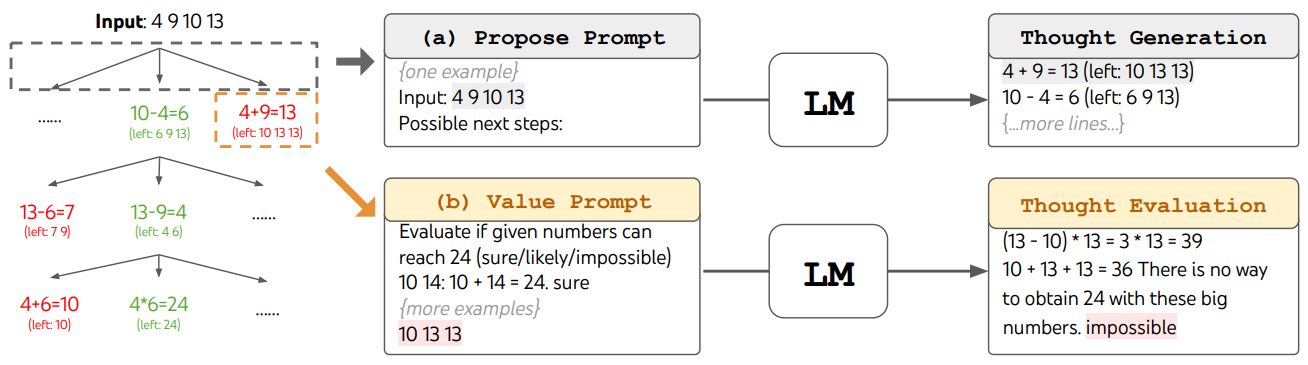
\includegraphics[height=0.8\textheight,width=\textwidth,keepaspectratio]{images/lrm+moe/tot-reasoning.png}
        \caption*{ToT in a game of 24. The LM is prompted for (a) thought generation and (b) valuation. Source: \href{https://arxiv.org/abs/2305.10601}{Yao et al. (2023)}}
    \end{figure}
    \framebreak
    \begin{figure}[h]
        \centering
        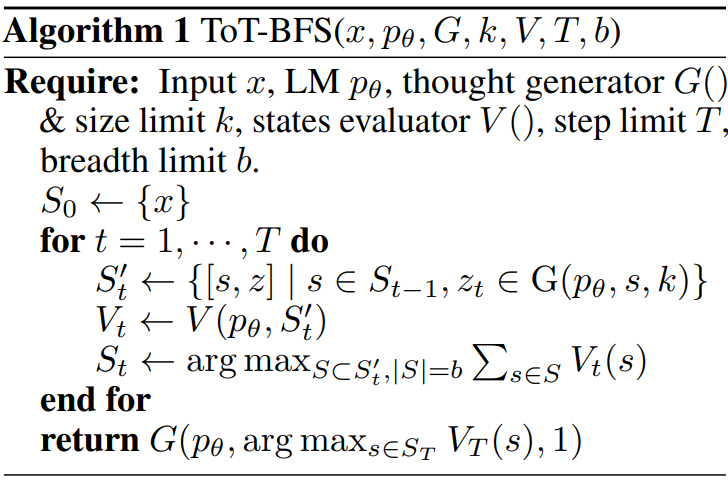
\includegraphics[height=0.9\textheight,width=\textwidth,keepaspectratio]{images/lrm+moe/algo-tot-bfs.png}
    \end{figure}
    \framebreak
    \begin{figure}[h]
        \centering
        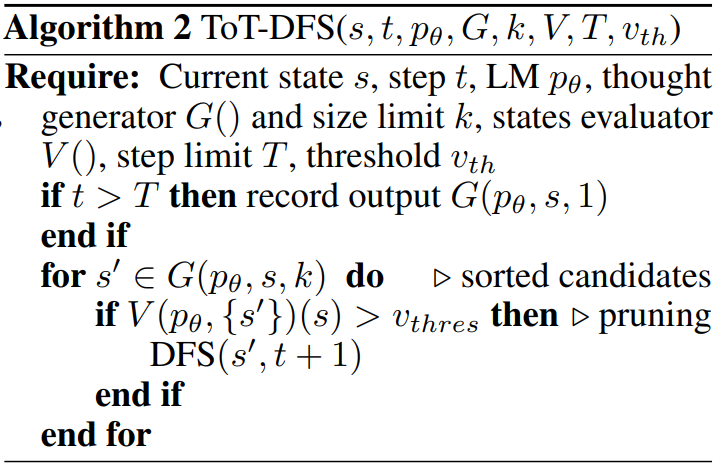
\includegraphics[height=0.9\textheight,width=\textwidth,keepaspectratio]{images/lrm+moe/algo-tot-dfs.png}
    \end{figure}
    \framebreak
    \begin{figure}[h]
        \centering
        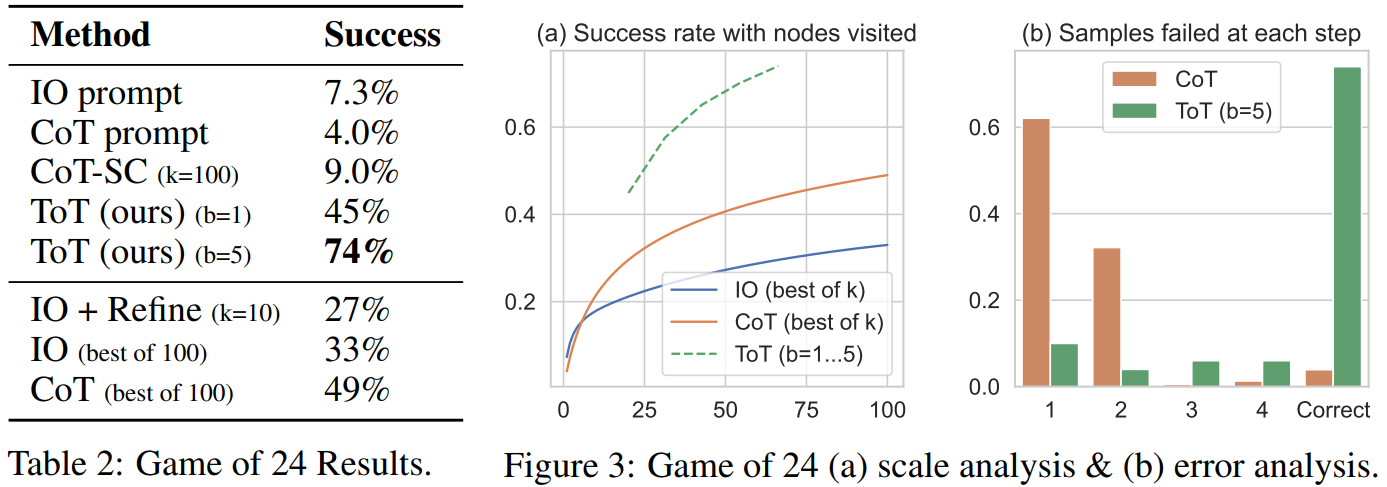
\includegraphics[height=0.9\textheight,width=\textwidth,keepaspectratio]{images/lrm+moe/tot-analysis+result.png}
    \end{figure}
    \framebreak
    \begin{figure}[h]
        \centering
        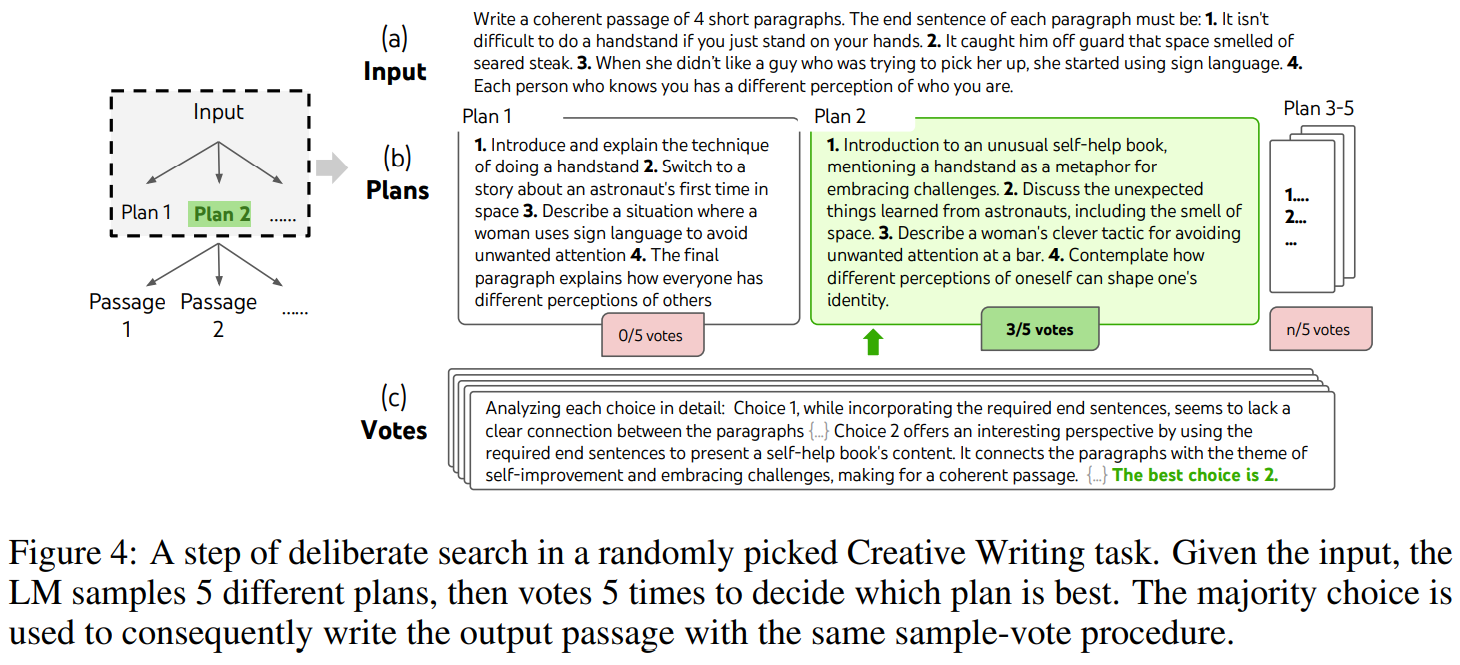
\includegraphics[height=0.9\textheight,width=\textwidth,keepaspectratio]{images/lrm+moe/tot-creative-writing-task.png}
    \end{figure}
    \framebreak
    \begin{figure}[h]
        \centering
        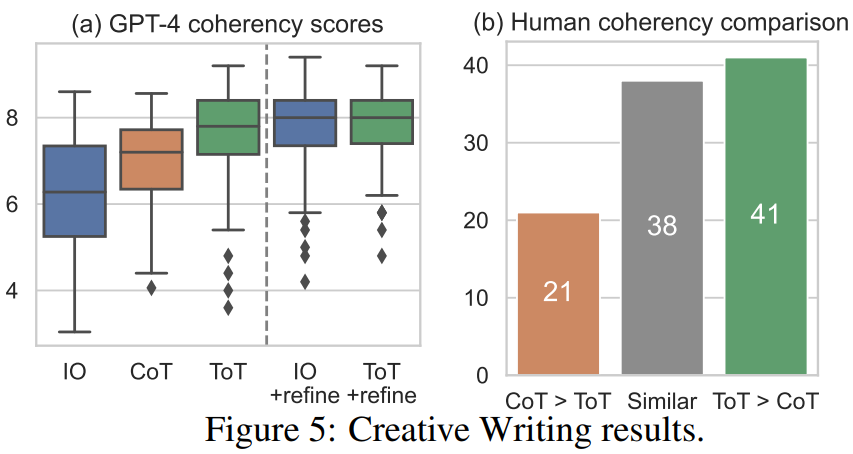
\includegraphics[height=0.9\textheight,width=\textwidth,keepaspectratio]{images/lrm+moe/tot-creative-writing-result.png}
    \end{figure}
\end{frame}


\subsection{Self-Consistency (SC)}
\begin{frame}[allowframebreaks]{Self-Consistency (SC)}
    \begin{figure}[h]
        \centering
        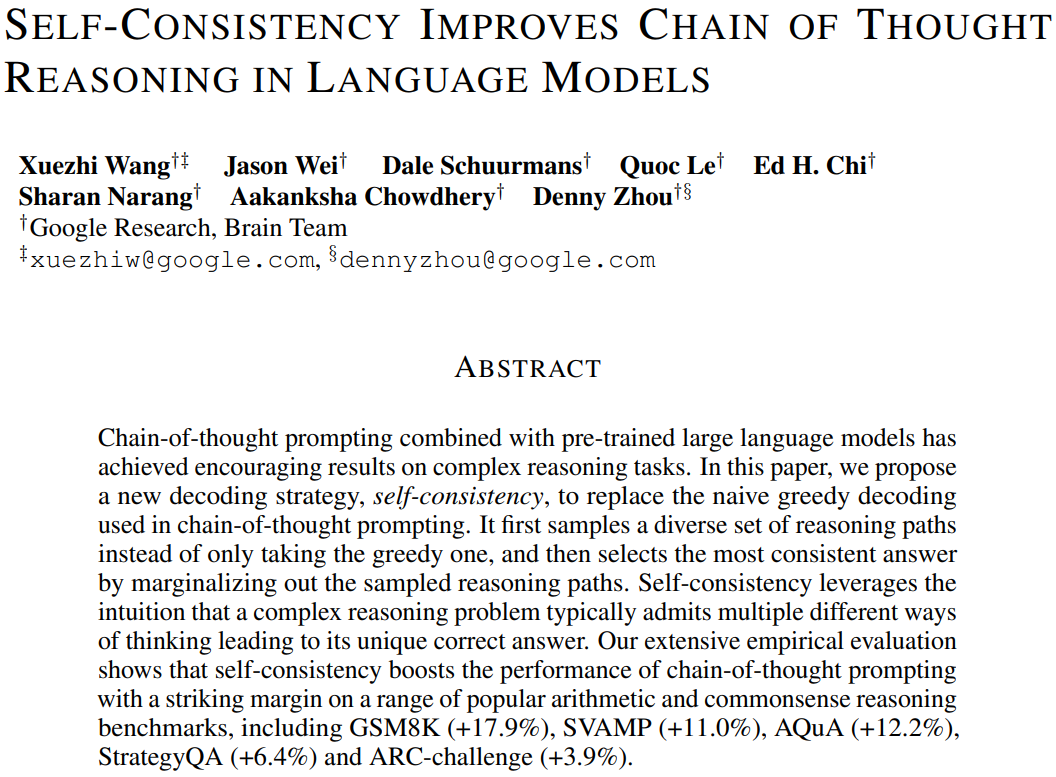
\includegraphics[height=0.9\textheight,width=\textwidth,keepaspectratio]{images/lrm+moe/paper-self-consistency.png}
    \end{figure}
    \begin{itemize}
        \item \textbf{What is Self-Consistency?}
        \begin{itemize}
            \item A technique that improves the reliability of LLM outputs by generating multiple responses to the same prompt and selecting the most consistent answer.
            \item Helps mitigate the variability in LLM responses, especially in tasks requiring reasoning or complex decision-making.
        \end{itemize}
        \item \textbf{How it works:}
        \begin{itemize}
            \item The model generates several responses to a given prompt.
            \item These responses are then evaluated for consistency, and the most frequent or coherent response is selected as the final answer.
        \end{itemize}
    \framebreak
        \item \textbf{Benefits:}
        \begin{itemize}
            \item Reduces the impact of noise and randomness in LLM outputs, leading to more reliable results.
            \item Enhances the model's performance on tasks that require stable and consistent reasoning.
        \end{itemize}
        \item \textbf{Example:}
        \begin{itemize}
            \item For a question like "What is the capital of France?", the model might generate multiple responses such as "Paris", "Paris is the capital", and "The capital city is Paris". The most consistent response ("Paris") would be selected as the final answer.
        \end{itemize}
    \end{itemize}
    \framebreak
    \begin{figure}[h]
        \centering
        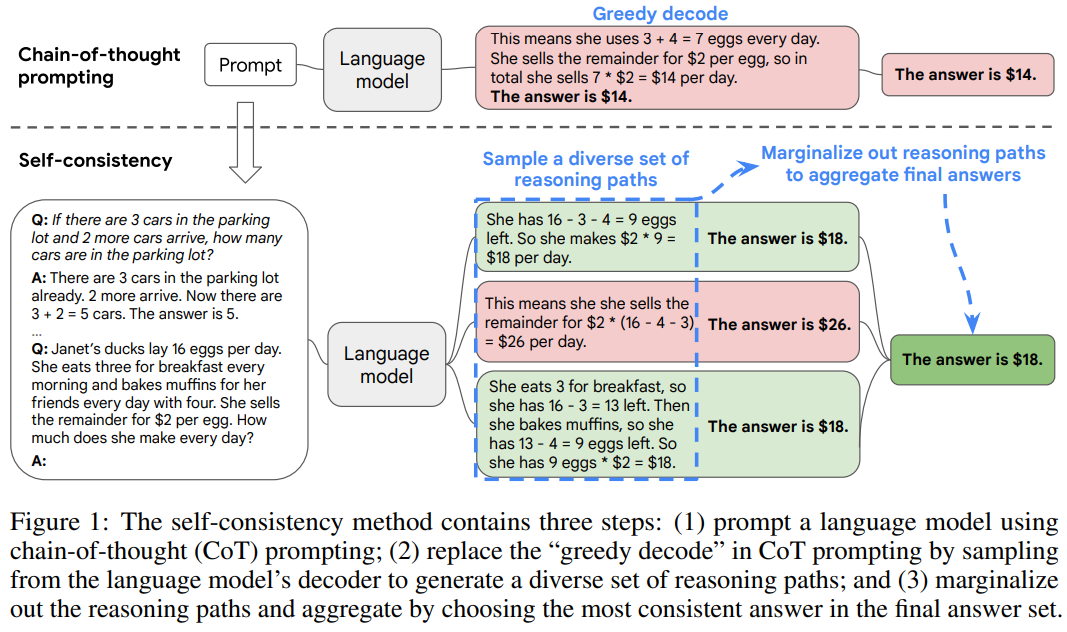
\includegraphics[height=0.8\textheight,width=\textwidth,keepaspectratio]{images/lrm+moe/self-consistency.png}
        \caption*{Source: \href{https://arxiv.org/abs/2203.11171}{Wang et al. (2022)}}
    \end{figure}
    \framebreak
    \begin{figure}[h]
        \centering
        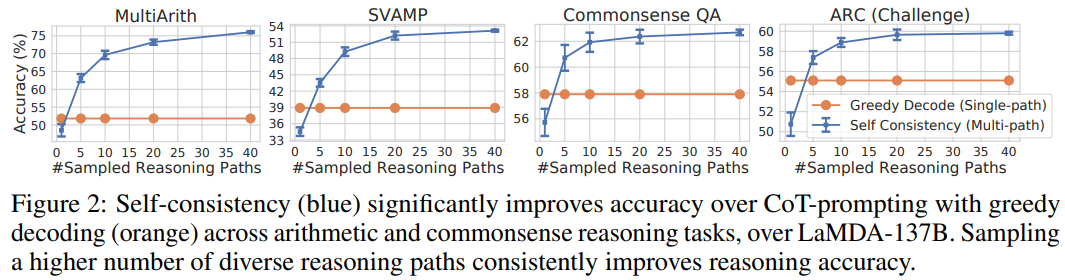
\includegraphics[height=0.9\textheight,width=\textwidth,keepaspectratio]{images/lrm+moe/self-consistency-accuracy.png}
    \end{figure}
    \framebreak
    \begin{figure}[h]
        \centering
        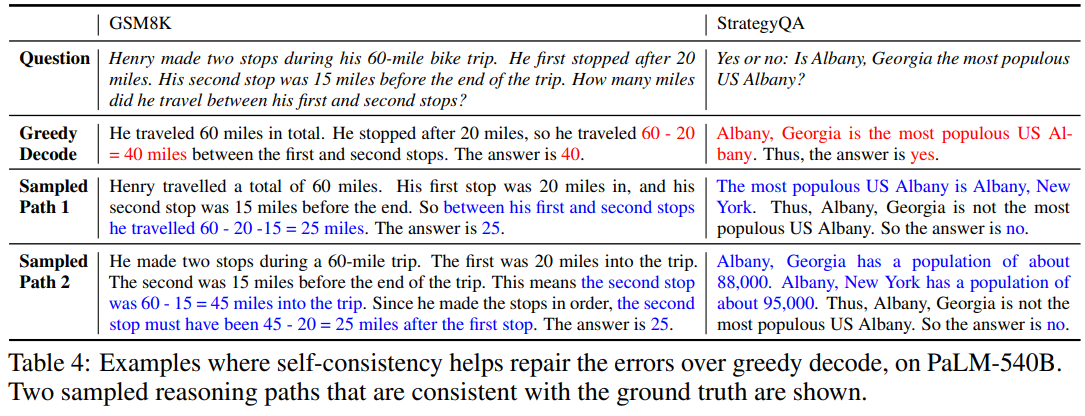
\includegraphics[height=0.9\textheight,width=\textwidth,keepaspectratio]{images/lrm+moe/self-consistency-benchmark.png}
    \end{figure}
    \framebreak
    \begin{figure}[h]
        \centering
        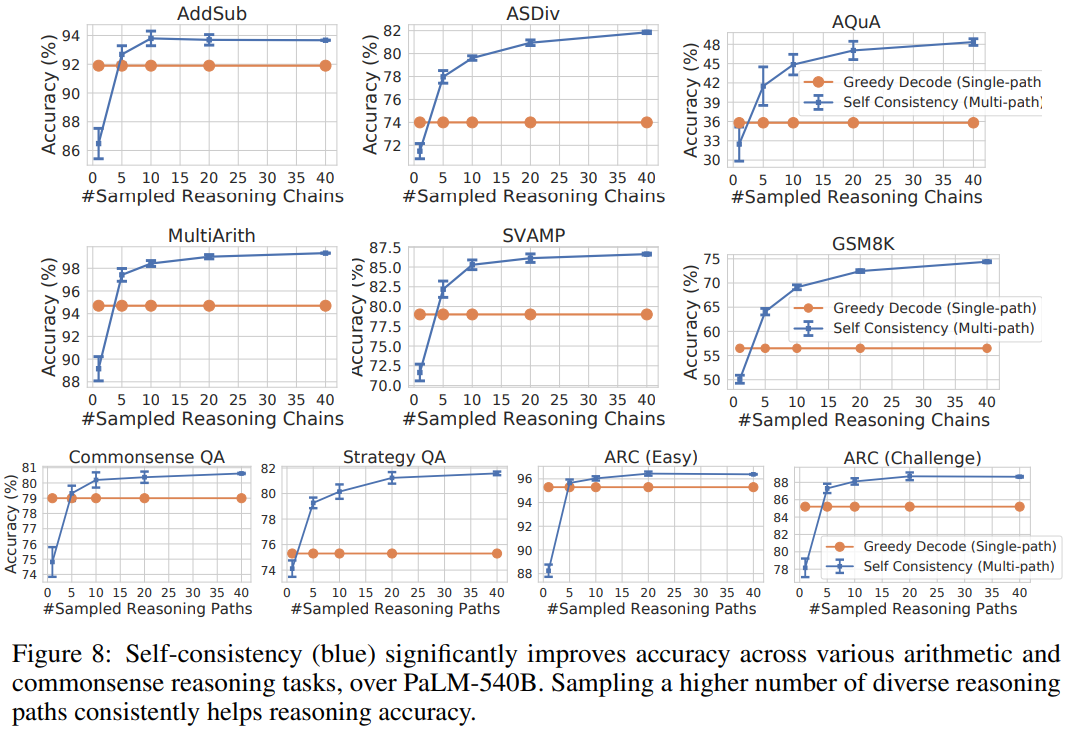
\includegraphics[height=0.9\textheight,width=\textwidth,keepaspectratio]{images/lrm+moe/self-consistency-accuracy-2.png}
    \end{figure}
\end{frame}